\section{Parallelization Methods}
    \subsection{POSIX Threads}
        \begin{frame}{PThreads - POSIX Threads}
            \begin{itemize}
                \item {
                    \textbf{POSIX} : Portable Operating System Interface for UNIX
                    }
                \item { Pthreads: The POSIX threading interface}
                \begin{itemize}
                \item {Thread implementations adhering to the POSIX standard}
                \item {System calls to create and synchronize threads}
                \item {Should be relatively uniform across UNIX-like OS platforms }
                \end{itemize}
             \item {Pthreads supports for }
             \begin{itemize}
             \item {Creating parallelism}
             \item {Synchronization}
             \end{itemize}
             \item {No explicit support for communication, because shared 
memory is implicit.}
            \end{itemize}
        \end{frame}
        

\subsection{CUDA}
\begin{frame}{Design Overview}

\begin{itemize}

\item{ Neural Network Training Steps }
\begin{itemize}
\item{\textbf{Forward propagation:}  \\$A_{i+1} = f(W_{i} \cdot A_{i})$}
\item{\textbf{Back propagation:}  \\$D_L =Y - A_L$,\\ $D_i = (W_{i})^{T}\cdot D_{i+1} \circ d(W_{i-1} \cdot A_{i-1})$}
\item{\textbf{Weight update:} \\$W_{i} = W_{i} + \frac{n}{b} \cdot \sum_{j=1}^{b} D_{i+1}^{j} \cdot A_{i}^j$}
\end{itemize}

\begin{center}
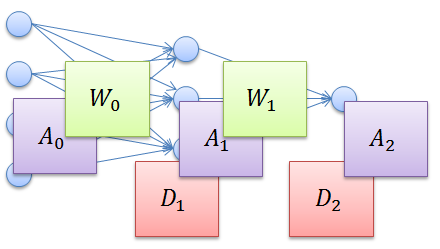
\includegraphics[width=2.4in]{gpu_neural_net_data.png}
\end{center}

\end{itemize}

\end{frame}

\begin{frame}{GPU Implementation Details}
\begin{itemize}
\item{Training Kernels}
\begin{itemize}
\item{ Variants of tiled matrix multiplication }
\item{ Each thread is responsible for computing a single matrix cell }
\item{ On-chip memory for amplifying }
\end{itemize}

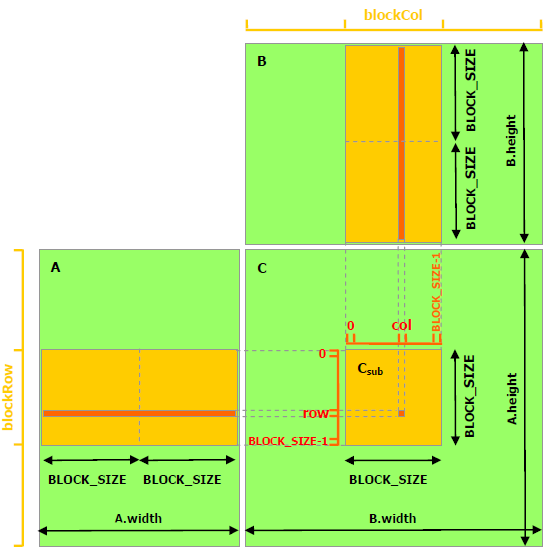
\includegraphics[width=2.0in]{matrix-multiplication-with-shared-memory.png}



\end{itemize}
\end{frame}

\begin{frame}{GPU Implementation Details (2)}
\begin{itemize}

\item{Optimization}
\begin{itemize}
\item{Coalesced access to global memory by iterating over the secondary dimension}
\item{Same strategy eliminates shared memory bank conflicts }
\end{itemize}

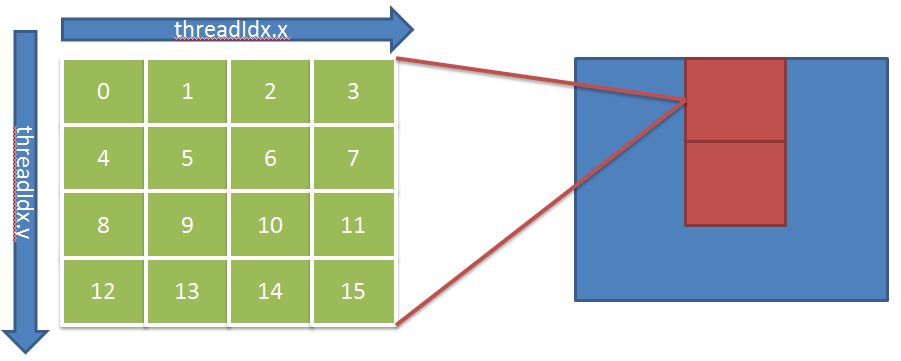
\includegraphics[width=3.0in]{gpu_mem_access.png}

\item{Neural Network Customization}
\begin{itemize}
\item{Single or double precision arithmetic}
\item{User preferred activation function}
\item{Abstract definition of network architecture and training parameters (i.e. batch size, learning rate) }

\end{itemize}


\end{itemize}
\end{frame}
    
